\documentclass[12pt]{article}
\parindent=.25in

\setlength{\oddsidemargin}{0pt}
\setlength{\textwidth}{440pt}
\setlength{\topmargin}{0in}

\usepackage[dvips]{graphicx}
\usepackage{amssymb}
\usepackage{amsfonts}
\usepackage{amsmath}

\DeclareMathOperator*{\argmax}{arg\,max}
\DeclareMathOperator*{\argmin}{arg\,min}

\title{Machine Learning Homework 2}
\author{Mengqi Zong $<mz2326@columbia.edu>$}

\begin{document}

\maketitle

\setlength{\parindent}{0in}

\section*{Problem 1}

The \textbf{E-step}
\begin{eqnarray*}
  Q(z_i)
  &=& p(z_i | x_i, \theta) \\
  &=& \frac {\pi_{z_i} p(x_i | \mu_{z_i})}
  {\sum_{z_i} \pi_{z_i} p(x_i | \mu_{z_i})} \\
  &=& \frac {\pi_{z_i} \prod_{j=1}^M \mu_{z_i}(j)^{x_i(j)}}
  {\sum_{z_p} \pi_{z_p} \prod_{q=1}^M \mu_{z_p}(p)^{x_i(q)}}
\end{eqnarray*}

The \textbf{M-step} \\

Let
\begin{equation*}
  Q_{i,t} (z_i) = p(z_i | x_i, \theta_t)
\end{equation*}

Based on the slides, we have
\begin{eqnarray*}
  Q(\theta | \theta_t)
  &=& \sum_{i=1}^N \sum_{z_i} p(z_i | x_i, \theta_t)
  \log {p(x_i, z_i | \theta)} \\
  &=& \sum_{i=1}^N \sum_{z_i} Q_{i,t}(z_i) \log {p(x_i, z_i | \theta)} \\
  &=& \sum_{i=1}^N  \sum_{z_i} Q_{i,t}(z_i)
  \log { \left( \pi_{z_i} \prod_{j=1}^M \mu_{z_i}(j)^{x_i(j)} \right) } \\
  &=& \sum_{i=1}^N \sum_{z_i} Q_{i,t}(z_i) \left(
    \log { \left( \pi_{z_i} \right)}
    + \sum_{j=1}^M x_i(j) \log { \left( \mu_{z_i}(j) \right)} \right)
\end{eqnarray*}

We know the constraint that for each $z_i = 1, 2, \dots, K$
\begin{eqnarray*}
  \sum_{j=1}^M \mu_{z_i}(j) = 1
\end{eqnarray*}

We also know the constraint that for each $z_i = 1, 2, \dots, K$
\begin{eqnarray*}
  \sum_{z_i} \pi_{z_i} = 1
\end{eqnarray*}


Combine $Q(\theta | \theta_t)$ with the previous constraint together, we get
\begin{eqnarray*}
  L(\theta) = \sum_{i=1}^N \sum_{z_i} Q_{i,t}(z_i) \left(
    \log { \left( \pi_{z_i} \right)}
    + \sum_{j=1}^M x_i(j) \log { \left( \mu_{z_i}(j) \right)} \right)
  + \alpha \left( \sum_{i=1}^N \sum_{j=1}^M \mu_{z_i}(j) - N \right)
  + \beta \left( \sum_{z_i} \pi_{z_i} - 1 \right)
\end{eqnarray*}

$L(\theta)$ taking the derivative with respect to $\mu_{z_i}(j)$, we get
\begin{eqnarray*}
  \frac {\partial \; L(\theta)} {\partial \; \mu_{z_i}(j)}
  &=& \frac {\partial} {\partial \; \mu_{z_i}(j)}
  \sum_{i=1}^N \sum_{z_i} Q_{i,t}(z_i) \left( \log { \left( \pi_{z_i} \right)}
      + \sum_{j=1}^M x_i(j) \log { \left( \mu_{z_i}(j) \right)} \right) \\
  && + \frac {\partial} {\partial \; \mu_{z_i}(j)} \left(
    \alpha \left( \sum_{i=1}^N \sum_{j=1}^M \mu_{z_i}(j) - N \right) \right)
    + \frac {\partial} {\partial \; \mu_{z_i}(j)} \left(
    \beta \left( \sum_{z_i} \pi_{z_i} - 1 \right) \right) \\
  &=& \sum_{i=1}^N Q_{i,t}(z_i) \frac {\partial} {\partial \; \mu_{z_i}(j)}
  \left( \log { \left( \pi_{z_i} \right)}
    + \sum_{j=1}^M x_i(j) \log { \left( \mu_{z_i}(j) \right)} \right)
  + \alpha \\
  &=& \sum_{i=1}^N Q_{i,t}(z_i) \frac {x_i(j)}{\mu_{z_i}(j)} + \alpha = 0 \\
  &\Rightarrow& \mu_{z_i}(j)
  = \frac {- \sum_{i=1}^N Q_{i,t}(z_i) x_i(j)}{\alpha} 
\end{eqnarray*}

Plug $\mu_{z_i}(j)$ back to the previous constraint, we get
\begin{eqnarray*}
  \sum_{j=1}^M \mu_{z_i}(j) &=& 1 \\
  \sum_{j=1}^M \frac {- \sum_{i=1}^N Q_{i,t}(z_i) x_i(j)}{\alpha} &=& 1 \\
  \alpha &=& - \sum_{i=1}^N \sum_{j=1}^M Q_{i,t}(z_i) x_i(j)
\end{eqnarray*}

Given $\alpha$, we get
\begin{eqnarray*}
  \mu_{z_i}(j)
  &=& \frac {- \sum_{i=1}^N Q_{i,t}(z_i) x_i(j)}{\alpha} \\
  &=& \frac {\sum_{i=1}^N Q_{i,t}(z_i) x_i(j)}
  {\sum_{i=1}^N \sum_{k=1}^M Q_{i,t}(z_i) x_i(k)} \\
  &=& \frac {\sum_{i=1}^N Q_{i,t}(z_i) x_i(j)}
  {\sum_{i=1}^N Q_{i,t}(z_i) \sum_{k=1}^M x_i(k)} \\
  &=& \frac {\sum_{i=1}^N Q_{i,t}(z_i) x_i(j)}
  {\sum_{i=1}^N Q_{i,t}(z_i)}
\end{eqnarray*}

$L(\theta)$ taking the derivative with respect to $\pi_{z_i}$, we get
\begin{eqnarray*}
  \frac {\partial \; L(\theta)} {\partial \; \pi_{z_i}}
  &=& \frac {\partial} {\partial \; \pi_{z_i}}
  \sum_{i=1}^N \sum_{z_i} Q_{i,t}(z_i) \left( \log { \left( \pi_{z_i} \right)}
      + \sum_{j=1}^M x_i(j) \log { \left( \mu_{z_i}(j) \right)} \right) \\
  && + \frac {\partial} {\partial \; \pi_{z_i}} \left(
    \alpha \left( \sum_{i=1}^N \sum_{j=1}^M \mu_{z_i}(j) - N \right) \right)
    + \frac {\partial} {\partial \; \pi_{z_i}} \left(
    \beta \left( \sum_{z_i} \pi_{z_i} - 1 \right) \right) \\
  &=& \sum_{i=1}^N Q_{i,t}(z_i) \frac {\partial} {\partial \; \pi_{z_i}}
  \left( \log { \left( \pi_{z_i} \right)}
    + \sum_{j=1}^M x_i(j) \log { \left( \mu_{z_i}(j) \right)} \right)
  + \beta \\
  &=& \sum_{i=1}^N Q_{i,t}(z_i) \frac {1}{\pi_{z_i}} + \beta = 0 \\
  &\Rightarrow& \pi_{z_i}
  = \frac {- \sum_{i=1}^N Q_{i,t}(z_i)}{\beta} 
\end{eqnarray*}

Plug $\pi_{z_i}$ back to the previous constraint, we get
\begin{eqnarray*}
  \sum_{z_i} \pi_{z_i} &=& 1 \\
  \sum_{z_i} \frac {- \sum_{i=1}^N Q_{i,t}(z_i)}{\beta} &=& 1 \\
  \beta &=& - \sum_{i=1}^N \sum_{z_i} Q_{i,t}(z_i)
\end{eqnarray*}

Given $\beta$, we get
\begin{eqnarray*}
  \pi_{z_i}
  &=& \frac {- \sum_{i=1}^N Q_{i,t}(z_i)}{\beta} \\
  &=& \frac {\sum_{i=1}^N Q_{i,t}(z_i)} {\sum_{i=1}^N \sum_{k} Q_{i,t}(k)} \\
  &=& \frac {\sum_{i=1}^N Q_{i,t}(z_i)} {N}
\end{eqnarray*}

To sum up, for $M$ step, we update $\theta$ as follow
\begin{eqnarray*}
  \mu_{z_i}(j)
  &=& \frac {\sum_{i=1}^N Q_{i,t}(z_i) x_i(j)}
  {\sum_{i=1}^N Q_{i,t}(z_i)}  \\
  \pi_{z_i}
  &=& \frac {\sum_{i=1}^N Q_{i,t}(z_i)} {N}
\end{eqnarray*}

\section*{Problem 2}

Note: for how to run the code, please refer to file ``running\_script.m''. \\


For this problem, all data will be 2-dimensional. \\

For the 4 clusters, the means are
\begin{eqnarray*}
  \mu_1 &=& (5, 5) \\
  \mu_2 &=& (0, 0) \\
  \mu_3 &=& (3, -3) \\
  \mu_4 &=& (-5, -5)
\end{eqnarray*}

All the covariance matrices are the same:
\begin{eqnarray*}
  \Sigma =
  \begin{pmatrix}
    1 & 0 \\
    0 & 1
  \end{pmatrix}
\end{eqnarray*}

The mixing proportions for each clusters from 1 to 4 are
\begin{eqnarray*}
  \pi = (0.3, 0.2, 0.1, 0.4)
\end{eqnarray*}

\textbf{Case $K = K_{true}$} \\

Here is one example of one data set and one clustering. The result is shown in Fig-\ref{fig:c1}. \\

\begin{figure}[ht!]
  \centering
  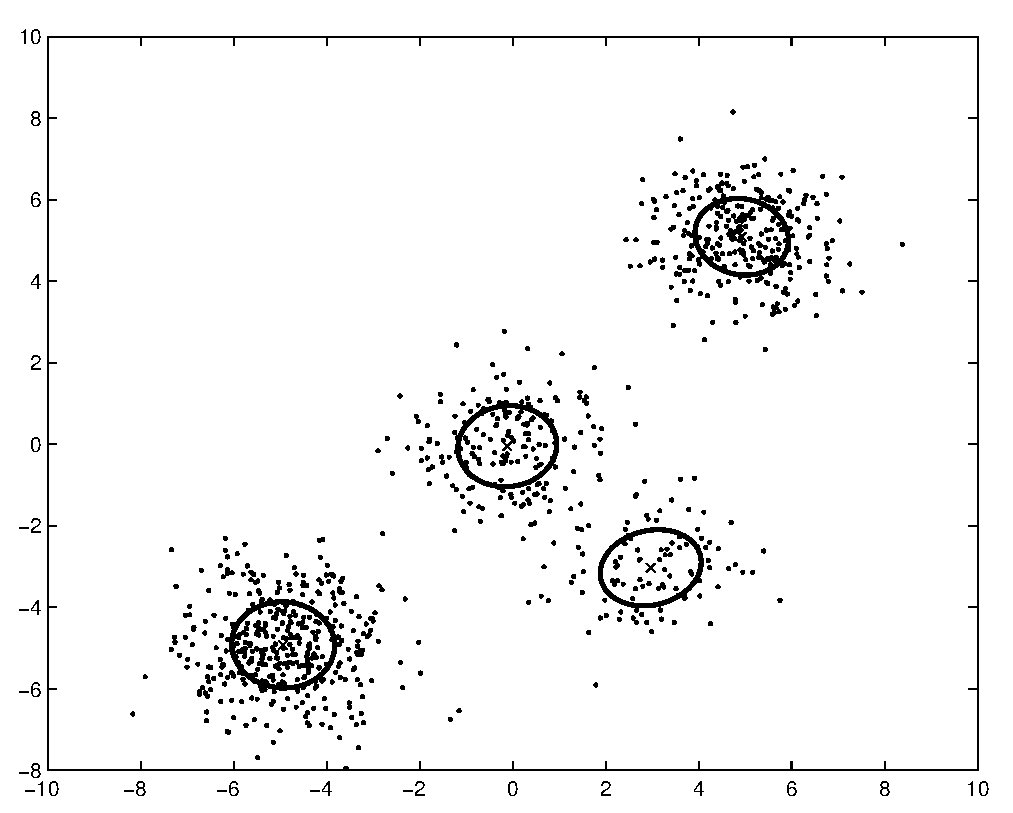
\includegraphics[width=0.7 \textwidth]{c1}
  \caption{$K = K_{true}$ \label{fig:c1}}
\end{figure}

And the estimated parameters are listed below
\begin{eqnarray*}
\hat{\mu_1} &=& (-0.1131,   -0.0468) \\
\hat{\mu_2} &=& (-4.9354,   -4.9216) \\
\hat{\mu_3} &=& (2.9710,   -3.0306) \\
\hat{\mu_4} &=& (4.9277,    5.0913) \\
\hat{\Sigma_1} &=&
  \begin{pmatrix}
    1.1309  &  0.0494 \\
    0.0494  &  0.9884
  \end{pmatrix} \\
\hat{\Sigma_2} &=& 
  \begin{pmatrix}
    1.2253  & -0.0254 \\
   -0.0254  &  1.1159
  \end{pmatrix} \\
\hat{\Sigma_3} &=&
  \begin{pmatrix}
    1.1790  &  0.1493 \\
    0.1493  &  0.8739
  \end{pmatrix} \\
\hat{\Sigma_4} &=& 
  \begin{pmatrix}
    1.0115  & -0.0813 \\
   -0.0813  &  0.8830
  \end{pmatrix} \\
\hat{\pi} &=& (0.1963, 0.4006, 0.1030, 0.3000)
\end{eqnarray*}

\textbf{Case $K > K_{true}$} \\

a) Example 1 \\

We will let $K = 5$. The initialized means for the 5 clusters are
\begin{eqnarray*}
\mu_{1_0} &=& (2.7567,   -2.3419) \\
\mu_{2_0} &=& (0.2141,    3.0156) \\
\mu_{3_0} &=& (6.6390,   -6.6342) \\
\mu_{4_0} &=& (-6.2178,    2.2398) \\
\mu_{5_0} &=& (4.6239,    7.2858)
\end{eqnarray*}

The result is shown in Fig-\ref{fig:c2-1}. \\

\begin{figure}[ht!]
  \centering
  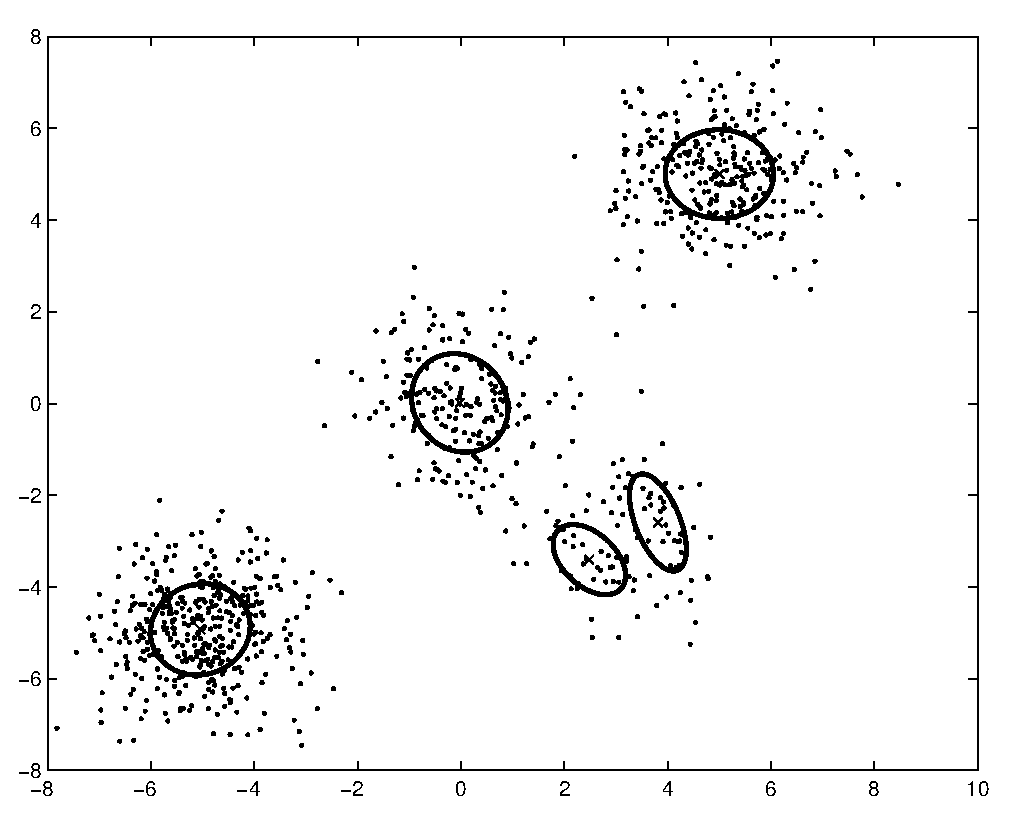
\includegraphics[width=0.7 \textwidth]{c2-1}
  \caption{$K = 5$ First Run \label{fig:c2-1}}
\end{figure}

And the estimated parameters are listed below
\begin{eqnarray*}
\hat{\mu_1} &=& (2.4849,   -3.4050) \\
\hat{\mu_2} &=& (-0.0225,    0.0140) \\
\hat{\mu_3} &=& (3.8133,   -2.5941) \\
\hat{\mu_4} &=& (-5.0444,   -4.9256) \\
\hat{\mu_5} &=& (5.0028,    5.0031) \\
\hat{\Sigma_1} &=&
  \begin{pmatrix}
    0.4919  & -0.2418 \\
   -0.2418  &  0.5845
  \end{pmatrix} \\
\hat{\Sigma_2} &=& 
  \begin{pmatrix}
    0.8721  & -0.1168 \\
   -0.1168  &  1.1525
  \end{pmatrix} \\
\hat{\Sigma_3} &=&
  \begin{pmatrix}
    0.3017  & -0.3207 \\
   -0.3207  &  1.1227
  \end{pmatrix} \\
\hat{\Sigma_4} &=& 
  \begin{pmatrix}
    0.9295  &  0.0660 \\
    0.0660  &  0.9922
  \end{pmatrix} \\
\hat{\Sigma_5} &=& 
  \begin{pmatrix}
    1.1040  & -0.0058 \\
   -0.0058  &  0.9363
  \end{pmatrix} \\
\hat{\pi} &=& (0.0459, 0.1996, 0.0536, 0.4000, 0.3008)
\end{eqnarray*}

For another run, the initialized means for the 5 clusters are
\begin{eqnarray*}
\mu_{1_0} &=& (6.8989,    6.3479) \\
\mu_{2_0} &=& (0.4094,    1.9085) \\
\mu_{3_0} &=& (3.8942,   -7.0989) \\
\mu_{4_0} &=& (1.5436,   -6.7613) \\
\mu_{5_0} &=& (-0.9384,   -0.4766)
\end{eqnarray*}

Then we get a different result, as shown in Fig-\ref{fig:c2-2}. \\

\begin{figure}[ht!]
  \centering
  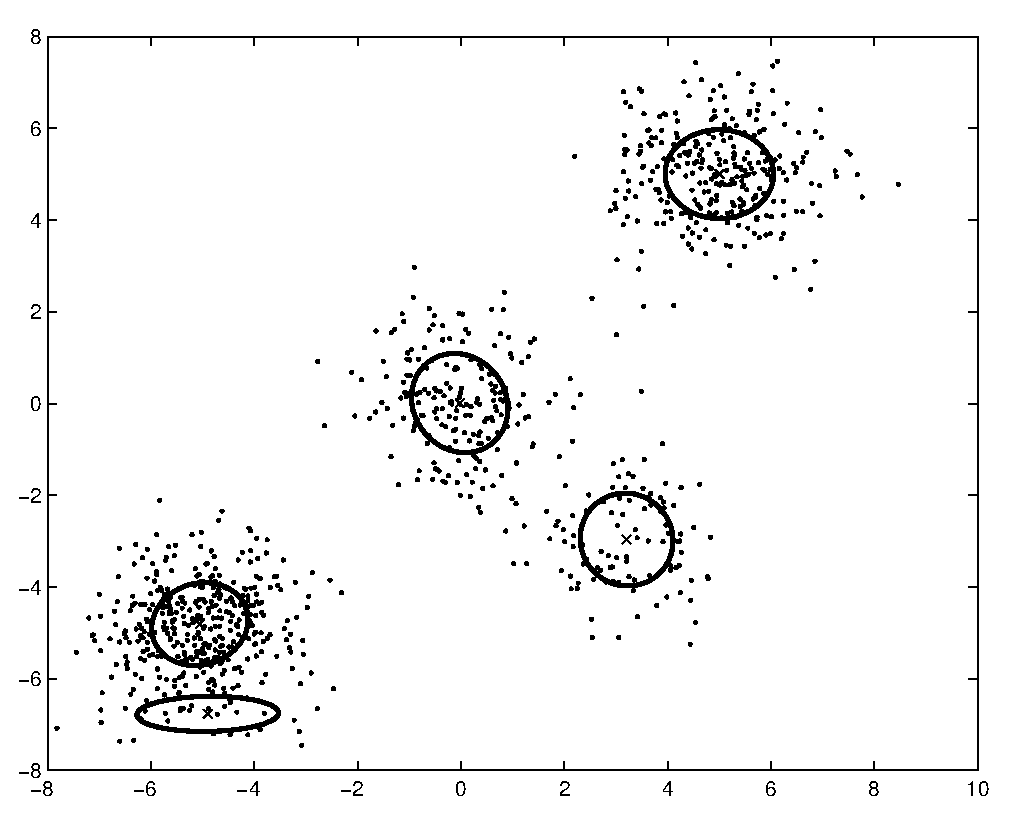
\includegraphics[width=0.7 \textwidth]{c2-2}
  \caption{$K = 5$ Second Run \label{fig:c2-2}}
\end{figure}

And the estimated parameters are listed below
\begin{eqnarray*}
\hat{\mu_1} &=& (5.0027,    5.0029) \\
\hat{\mu_2} &=& (-0.0231,    0.0105) \\
\hat{\mu_3} &=& (3.2069,   -2.9669) \\
\hat{\mu_4} &=& (-4.9020,   -6.7690) \\
\hat{\mu_5} &=& (-5.0534,   -4.8094) \\
\hat{\Sigma_1} &=&
  \begin{pmatrix}
    1.1041  & -0.0054 \\
   -0.0054  &  0.9371
  \end{pmatrix} \\
\hat{\Sigma_2} &=& 
  \begin{pmatrix}
    0.8710  & -0.1136 \\
   -0.1136  &  1.1710
  \end{pmatrix} \\
\hat{\Sigma_3} &=&
  \begin{pmatrix}
    0.8064  & -0.0264 \\
   -0.0264  &  1.0245
  \end{pmatrix} \\
\hat{\Sigma_4} &=& 
  \begin{pmatrix}
    1.8770  &  0.0289 \\
    0.0289  &  0.1465
  \end{pmatrix} \\
\hat{\Sigma_5} &=& 
  \begin{pmatrix}
    0.8684  &  0.0860 \\
    0.0860  &  0.8178
  \end{pmatrix} \\
\hat{\pi} &=& ( 0.3008, 0.1998, 0.0994, 0.0237, 0.3763)
\end{eqnarray*}

b) Example 2 ($K = 6$) \\

We will let $K = 6$. For the first run, the initialized means for the 6 clusters are
\begin{eqnarray*}
\mu_{1_0} &=& (-0.2314,   -4.0058) \\
\mu_{2_0} &=& (2.9457,    4.3839) \\
\mu_{3_0} &=& (-7.4056,   -4.8665) \\
\mu_{4_0} &=& (-5.4095,    1.8251) \\
\mu_{5_0} &=& (3.0565,    5.3207) \\
\mu_{6_0} &=& (-8.4153,   -5.1901)
\end{eqnarray*}

The result is shown in Fig-\ref{fig:c2-3}. \\

\begin{figure}[ht!]
  \centering
  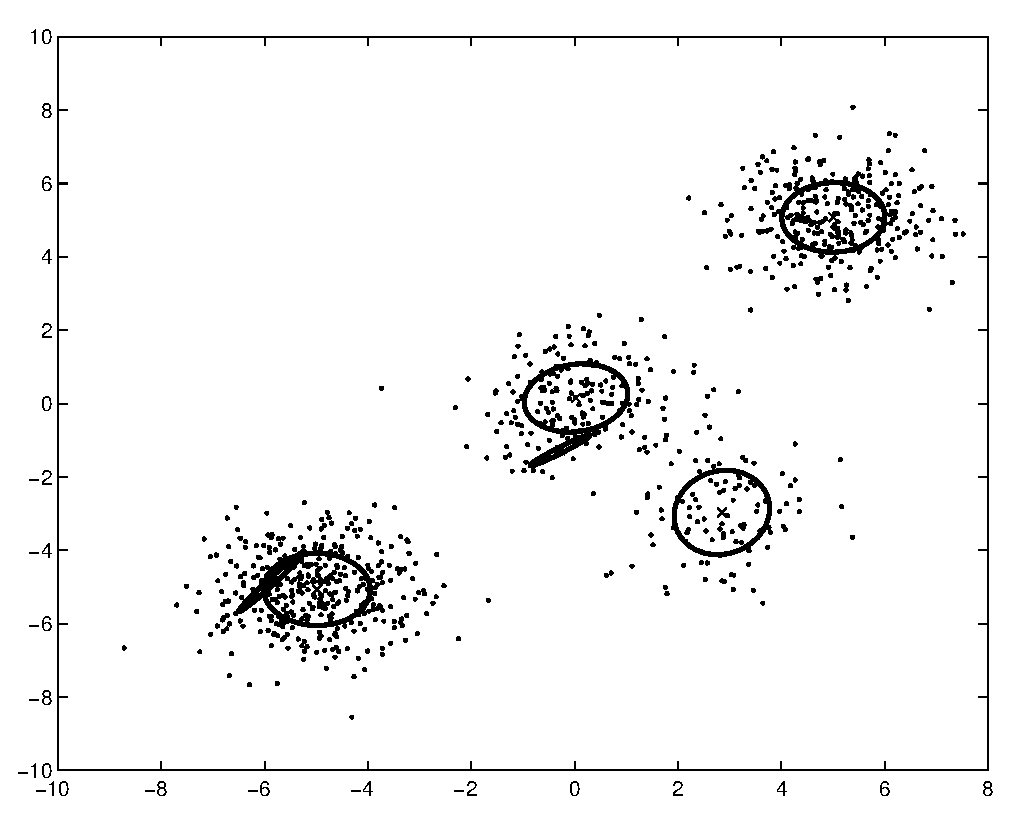
\includegraphics[width=0.7 \textwidth]{c2-3}
  \caption{$K = 6$ First Run \label{fig:c2-3}}
\end{figure}

For the second run, the initialized means for the 6 clusters are
\begin{eqnarray*}
\mu_{1_0} &=& (0.8004,    7.5505) \\
\mu_{2_0} &=& (0.7264,   -6.8910) \\
\mu_{3_0} &=& (-6.0163,   -6.8529) \\
\mu_{4_0} &=& (-6.3469,    2.6142) \\
\mu_{5_0} &=& (1.6702,   -2.3586) \\
\mu_{6_0} &=& (-6.0768,   -2.0746)
\end{eqnarray*}

The result is shown in Fig-\ref{fig:c2-4}. \\

\begin{figure}[ht!]
  \centering
  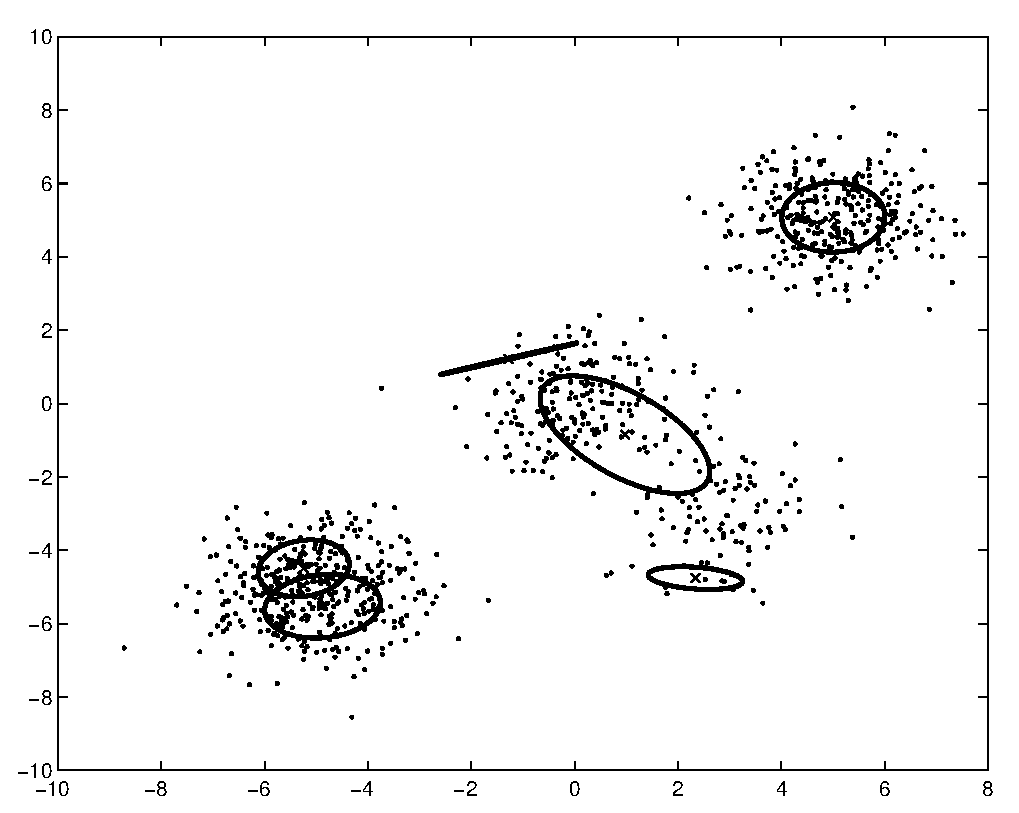
\includegraphics[width=0.7 \textwidth]{c2-4}
  \caption{$K = 6$ Second Run \label{fig:c2-4}}
\end{figure}

\textbf{Case $K < K_{true}$} \\

a) Unstable case \\

As usual, we will use the means, variances and mixing proportions defined at the beginning of the answer. We will let $K = 2$. And we find that the results are unstable.

For the first run, the initialized means for the 2 clusters are
\begin{eqnarray*}
\mu_{1_0} &=& (1.9731,    4.6843) \\
\mu_{2_0} &=& (-6.1752,    7.7035)
\end{eqnarray*}

The result is shown in Fig-\ref{fig:c3-1}. \\

\begin{figure}[ht!]
  \centering
  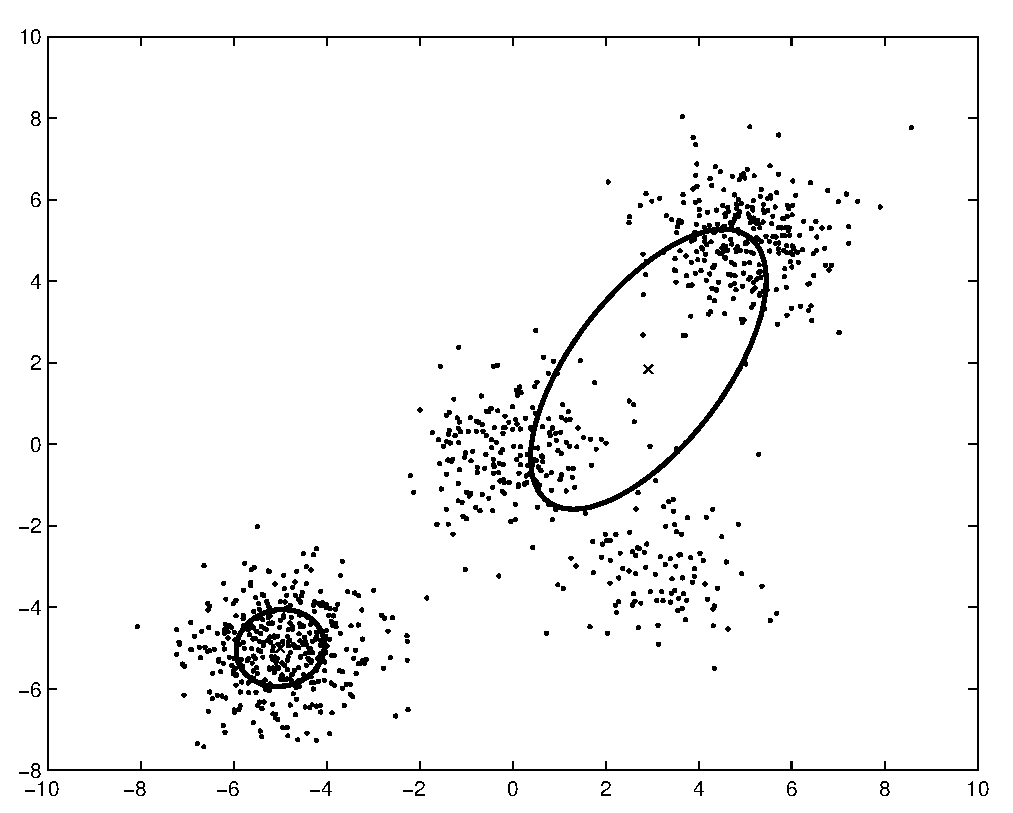
\includegraphics[width=0.7 \textwidth]{c3-1}
  \caption{$K = 2$ Unstable: First Run \label{fig:c3-1}}
\end{figure}

The estimated parameters are listed below
\begin{eqnarray*}
\hat{\mu_1} &=& (2.9212,    1.8428) \\
\hat{\mu_2} &=& (-4.9980,   -4.9982) \\
\hat{\Sigma_1} &=&
  \begin{pmatrix}
    6.4136  &  5.5430 \\
    5.5430  & 11.7903
  \end{pmatrix} \\
\hat{\Sigma_2} &=& 
  \begin{pmatrix}
    0.9033  &  0.0572 \\
    0.0572  &  0.8967
  \end{pmatrix} \\
\hat{\pi} &=& (0.6098, 0.3902)
\end{eqnarray*}

For the second run, the initialized means for the 2 clusters are
\begin{eqnarray*}
\mu_{1_0} &=& (-7.2031,   -4.0285) \\
\mu_{2_0} &=& (-0.4189,    7.3939)
\end{eqnarray*}

The result is shown in Fig-\ref{fig:c3-2}. \\

\begin{figure}[ht!]
  \centering
  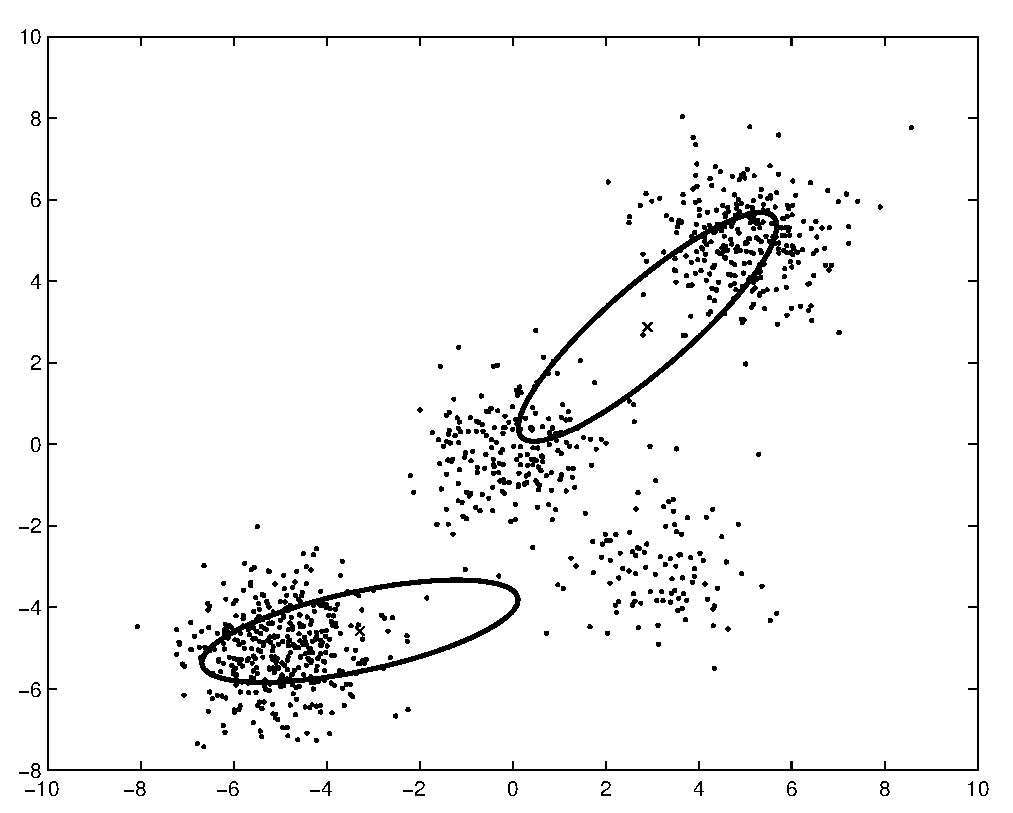
\includegraphics[width=0.7 \textwidth]{c3-2}
  \caption{$K = 2$ Unstable: Second Run \label{fig:c3-2}}
\end{figure}

And the estimated parameters are listed below
\begin{eqnarray*}
\hat{\mu_1} &=& (-3.2826,   -4.5848) \\
\hat{\mu_2} &=& (4.4624,    2.9207) \\
\hat{\Sigma_1} &=&
  \begin{pmatrix}
   11.5557  &  2.6195 \\
    2.6195  &  1.5741
  \end{pmatrix} \\
\hat{\Sigma_2} &=& 
  \begin{pmatrix}
    7.7172  &  6.8535 \\
    6.8535  &  7.8699
  \end{pmatrix} \\
\hat{\pi} &=& (0.4966, 0.5034)
\end{eqnarray*}

b) Stable case \\

For the stable case, we will use new parameters
For the 4 clusters, the means are
\begin{eqnarray*}
  \mu_1 &=& (3, 4) \\
  \mu_2 &=& (4, 3) \\
  \mu_3 &=& (-3, -4) \\
  \mu_4 &=& (-4, -3)
\end{eqnarray*}

All the covariance matrices are the same:
\begin{eqnarray*}
  \Sigma =
  \begin{pmatrix}
    1 & 0 \\
    0 & 1
  \end{pmatrix}
\end{eqnarray*}

The mixing proportions for each clusters from 1 to 4 are all equal. That is,
\begin{eqnarray*}
  \pi = (0.25, 0.25, 0.25, 0.25)
\end{eqnarray*}

Then we will get stable results. One result is shown in Fig-\ref{fig:c3-3}. \\

\begin{figure}[ht!]
  \centering
  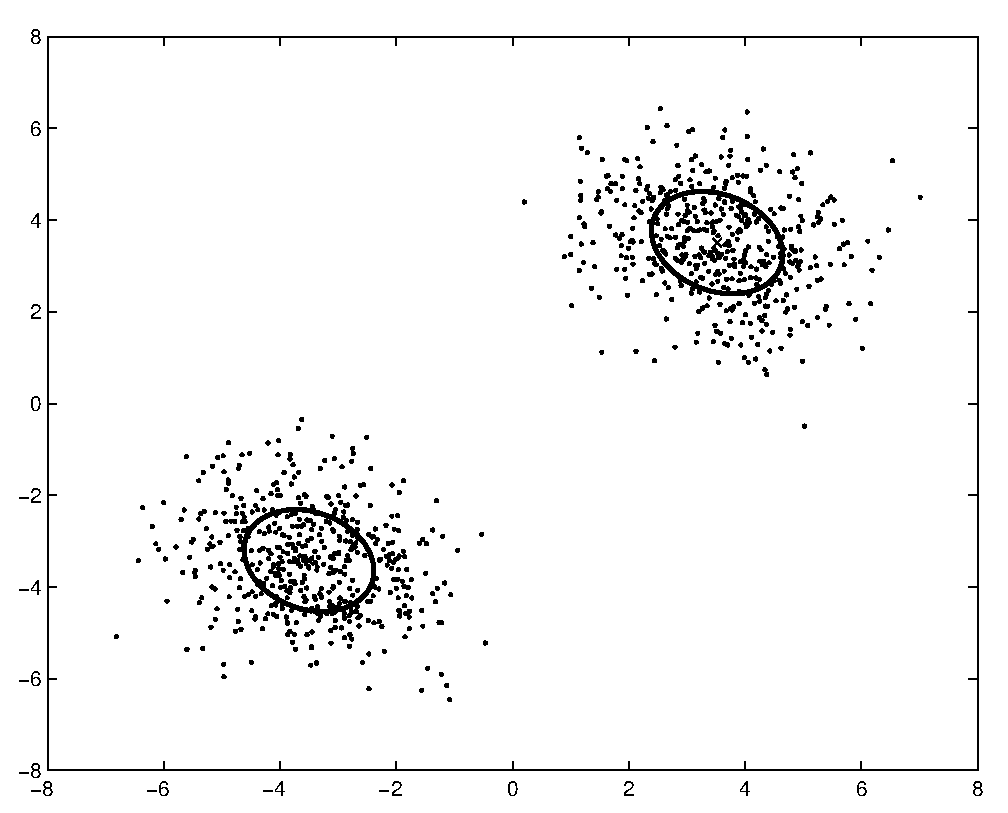
\includegraphics[width=0.7 \textwidth]{c3-3}
  \caption{$K = 2$ Stable \label{fig:c3-3}}
\end{figure}

The estimated parameters are listed below
\begin{eqnarray*}
\hat{\mu_1} &=& (3.5196,    3.5090) \\
\hat{\mu_2} &=& (-3.5037,   -3.4241) \\
\hat{\Sigma_1} &=&
  \begin{pmatrix}
    1.2762  & -0.2912 \\
   -0.2912  &  1.2448
  \end{pmatrix} \\
\hat{\Sigma_2} &=& 
  \begin{pmatrix}
    1.2471  & -0.2553 \\
   -0.2553  &  1.2320
  \end{pmatrix} \\
\hat{\pi} &=& (0.5000, 0.5000)
\end{eqnarray*}

\section*{Problem 3}

a) \\
Let $x_1, x_2, \dots, x_n$ be $n$ non-negative numbers.
\begin{eqnarray*}
  Mean_{arithmetic} &=& \frac{1}{n} \sum_{i=1}^n x_i \\
  Mean_{geometric} &=& \sqrt[n] {x_1x_2 \dots x_n}
\end{eqnarray*}

Then we have
\begin{eqnarray*}
  \ln { \left( Mean_{arithmetic} \right) }
  &=& \ln { \left( \frac{1}{n} \sum_{i=1}^n x_i \right) } \\
  &\ge& \sum_{i=1}^n \frac{1}{n} \ln {  x_i } \\
  &=& \ln { \left( \sqrt[n] {x_1x_2 \dots x_n} \right) } \\
  &=& \ln { \left( Mean_{geometric} \right) }
\end{eqnarray*}

So, the arithmetic mean of non-negative numbers is at least their geometric mean. \\

b) \\
We will begin our proof from the right side of the inequality.
\begin{eqnarray*}
  \exp { \left( \theta^T \sum_{i=1}^m \alpha_i f_i
    - \sum_{i=1}^m \alpha_i \log {\alpha_i} \right) }
  &=& \exp { \left( \sum_{i=1}^m \alpha_i (\theta^T f_i - \log {\alpha_i})
    \right) } \\
  &\le& \sum_{i=1}^m \alpha_i \exp { \left( 
      \theta^T f_i - \log {\alpha_i} \right) } \\
  &=& \sum_{i=1}^m \alpha_i \exp { \left( \theta^T f_i \right) }
  \frac {1}{\alpha_i} \\
  &=& \sum_{i=1}^m \exp { \left( \theta^T f_i \right) }
\end{eqnarray*}

\end{document}
